\subsection{Latent Space Models}
\label{sec:Method:LSM}
This subsection delves with explaining and understanding the latent space modelling approach.

A latent space, also refereed to as a latent embedding space, serves as an embedding in which a set of entities, in this project the nodes of a dynamic network, who resemble each other more closely are positioned closer in the latent space \cite{Sarkar2005DynamicModels} \cite{Kim2017AVariables}.
For a given set of four nodes, with weighted links between them, this weight can be represented in two-dimensional latent space by their reciprocal distances.  

\begin{figure}[H]
    \centering
    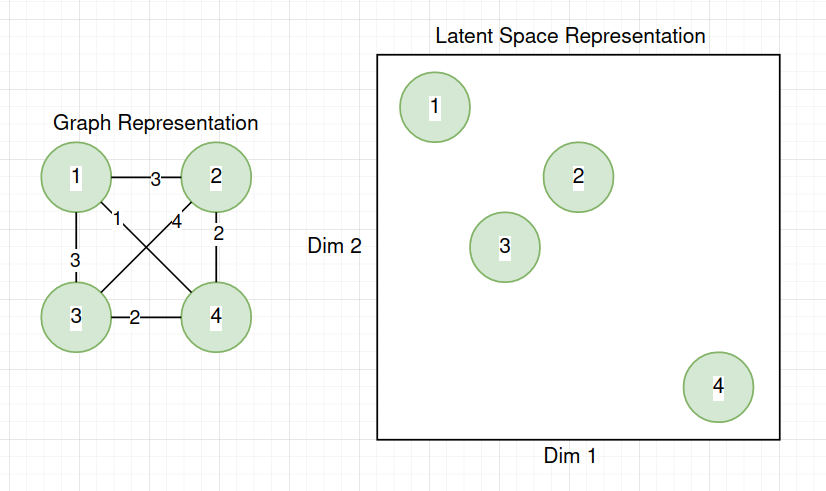
\includegraphics[width=0.8\textwidth]{0_images/latentspace.png}
    \caption{Four nodes placed in two-dimensional latent space, weights represented by their reciprocal distances.}
    \label{fig:latentspace}
\end{figure}
For this project, the resemblance of nodes, shown as the link weights in figure \ref{fig:latentspace}, is based on the intensity of interaction between entities in a given dynamic network.
This intensity is defined by the intensity function, which is described later in section \ref{sec:Method:IntensityFunc}.

The latent space, being a two-dimensional space, serves as a dimensionality reduction, given the fact that the dynamics of the networks which are being mapped are of possibly much higher dimensions.
Latent space models, or latent distance models as they are also referred to, have proved good in modelling higher dimensional data in lower dimensions \cite{Gourieroux2021ScalableNetworks}.

As mentioned in section \ref{sec:Intro:RelatedWork} about related work, the latent space approach by Sarkar and Moore et. al. modelled dynamic networks using only positions in latent space \cite{Sarkar2005DynamicModels}.
Tomerup et. al. \cite{Tommerup2021LearningNetworks} expanded their modelling approach by attributing the nodes of a dynamic network with simple Newtonian dynamics of motion, and even though most dynamic networks are not be governed by Newtonian dynamics, this approach has the advantage of having a higher degree of explainability.
This project expands the capabilities of the Newtonian dynamics approach, in order to better model dynamic networks which are not Newtonian in nature.


\subsubsection{Euclidean Latent Space}
\label{sec:Method:LSM:EuclideanLatentSpace}
The Euclidean latent space is governed by Euclidean geometry in two dimensions.
This means any measure of position, distance and velocity are understood as Euclidean and can be computed as such. 
Taking an offset in the nodes of a dynamic network, and the modelling approach of presented in this project, the properties of Euclidean space will be explained below.
\\\\
Given a dynamic network consisting of $N$ nodes, these are all placed in the Euclidean latent space. 
Positions in the Euclidean latent space are denoted as two-dimensional coordinates, and hence each node in the given network is assigned a position, expressed for node $u$ as
$\textbf{z}_u = \begin{pmatrix}
x_u, y_u
\end{pmatrix}^T$.

As the project deals with temporally dynamic networks specifically, the positions of nodes are temporally dependant. 
In order to accommodate for this, each node is assigned one or more velocity vectors, which entails that they move along the trajectory of a constant velocity over a given timespan.
For node $u$, the velocity vector is expressed as:
$\textbf{v}_u = \begin{pmatrix}
v_{x,u}, v_{y,u}
\end{pmatrix}^T$.

By having a starting position, $\textbf{z}_u$, as well as a constant velocity, $\textbf{v}_u$, the position of a node at any time, $t$, is given by: 

\begin{equation}
    \textbf{z}_u(t) = \begin{pmatrix}
    x_u\\
    y_u
    \end{pmatrix}
    +
    \begin{pmatrix}
    v_{x,u}\\
    v_{y,u}
    \end{pmatrix}
    t
    = 
    \begin{pmatrix}
    x_u + v_{x,u}t\\
    y_u + v_{y,u}t
    \label{eq:latent_pos}
    \end{pmatrix}
\end{equation}
In the Euclidean latent space, based on the given positions, it is possible to compute distances using basic Pythagorean mathematics. 
In order to find the distance between two nodes, the most straightforward approach is to compute their reciprocal Euclidean distance.
The Euclidean distance at the starting position, ie. disregarding time, between nodes $u$ and $v$, can be computed from the following expression:

\begin{equation}
    ||\textbf{z}_u - \textbf{z}_v||_2
    = 
    \sqrt{(x_u - x_v)^2 + (y_u - y_v)^2}
\end{equation}
As mentioned above though, the positions of nodes are in fact time dependant, and hence this carries over to the distance measure, which is expressed as:

\begin{equation}
    ||\textbf{z}_u(t) - \textbf{z}_v(t)||_2
    = 
    \sqrt{((x_u + v_{x,u}t) - (x_v + v_{x,v}t))^2 + ((y_u + v_{y,u}t) - (y_v + v_{y,v}t))^2}
\end{equation}
For mathematical and computational reasons, which are explained in detail under section \ref{sec:Method:IntensityFunc:IntegralIntensityFunc}, this project utilizes the squared Euclidean distance as distance measure.
This is written below, in a simplified form:

\begin{equation} 
||\textbf{z}_u(t) - \textbf{z}_v(t)||_2^2
= 
(x_u - x_v + (v_{x,u} - v_{x,v})t)^2 + (y_u - y_v + ( v_{y,u} - v_{y,v})t)^2
\label{eq:SquaredEuclideanDistance}
\end{equation}



